For part two in this lab, the database application was tested using the bottom
up incremental testing strategy. Unit tests were made starting at the lower
level modules, building our way up to the higher level modules so that nothing
was mocked. The
actual tests can be found in Appendix \ref{bottumup}, and are also in the zip
archive in which this report was submitted. They can be found in
\emph{``Lab 5/Lab 5/src/test/java/bottumup''} The test results are found on the
next page.
%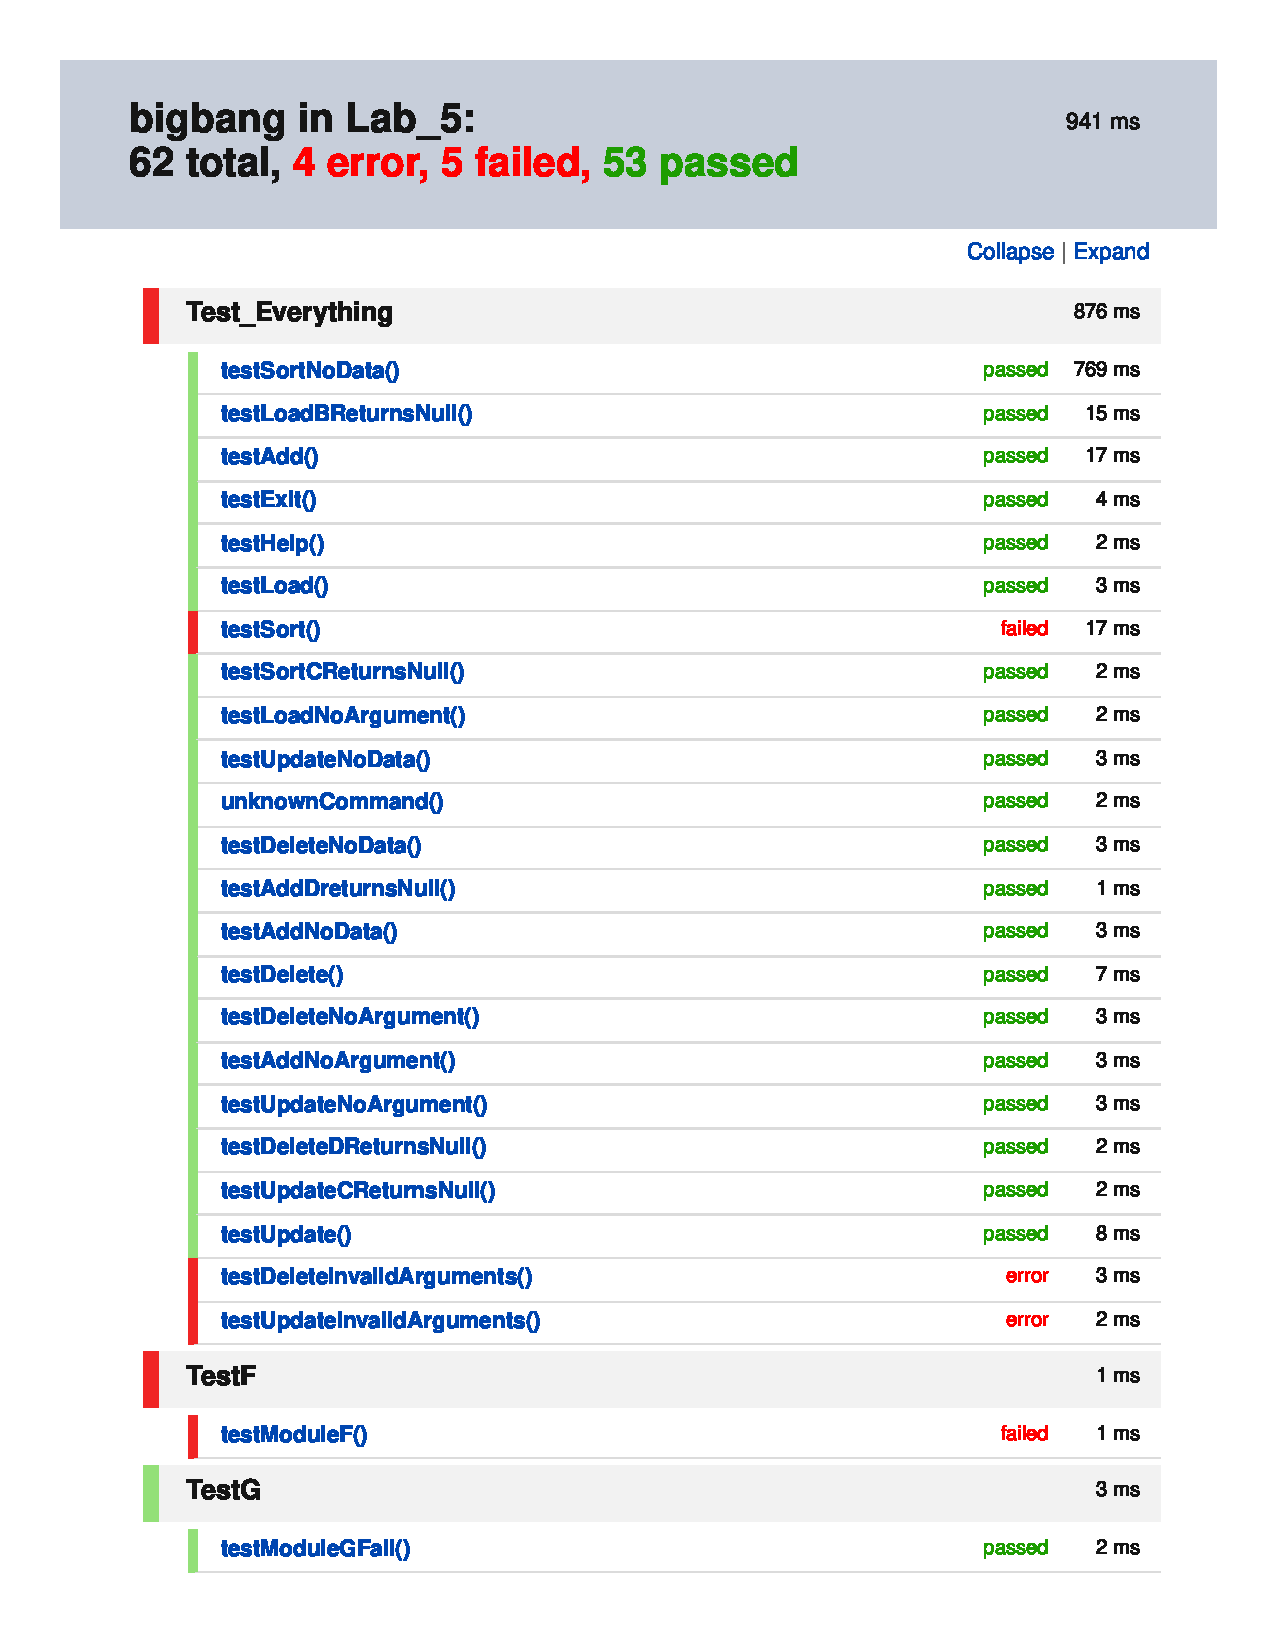
\includepdf[pages=-]{resources/bigbang_results.pdf}
%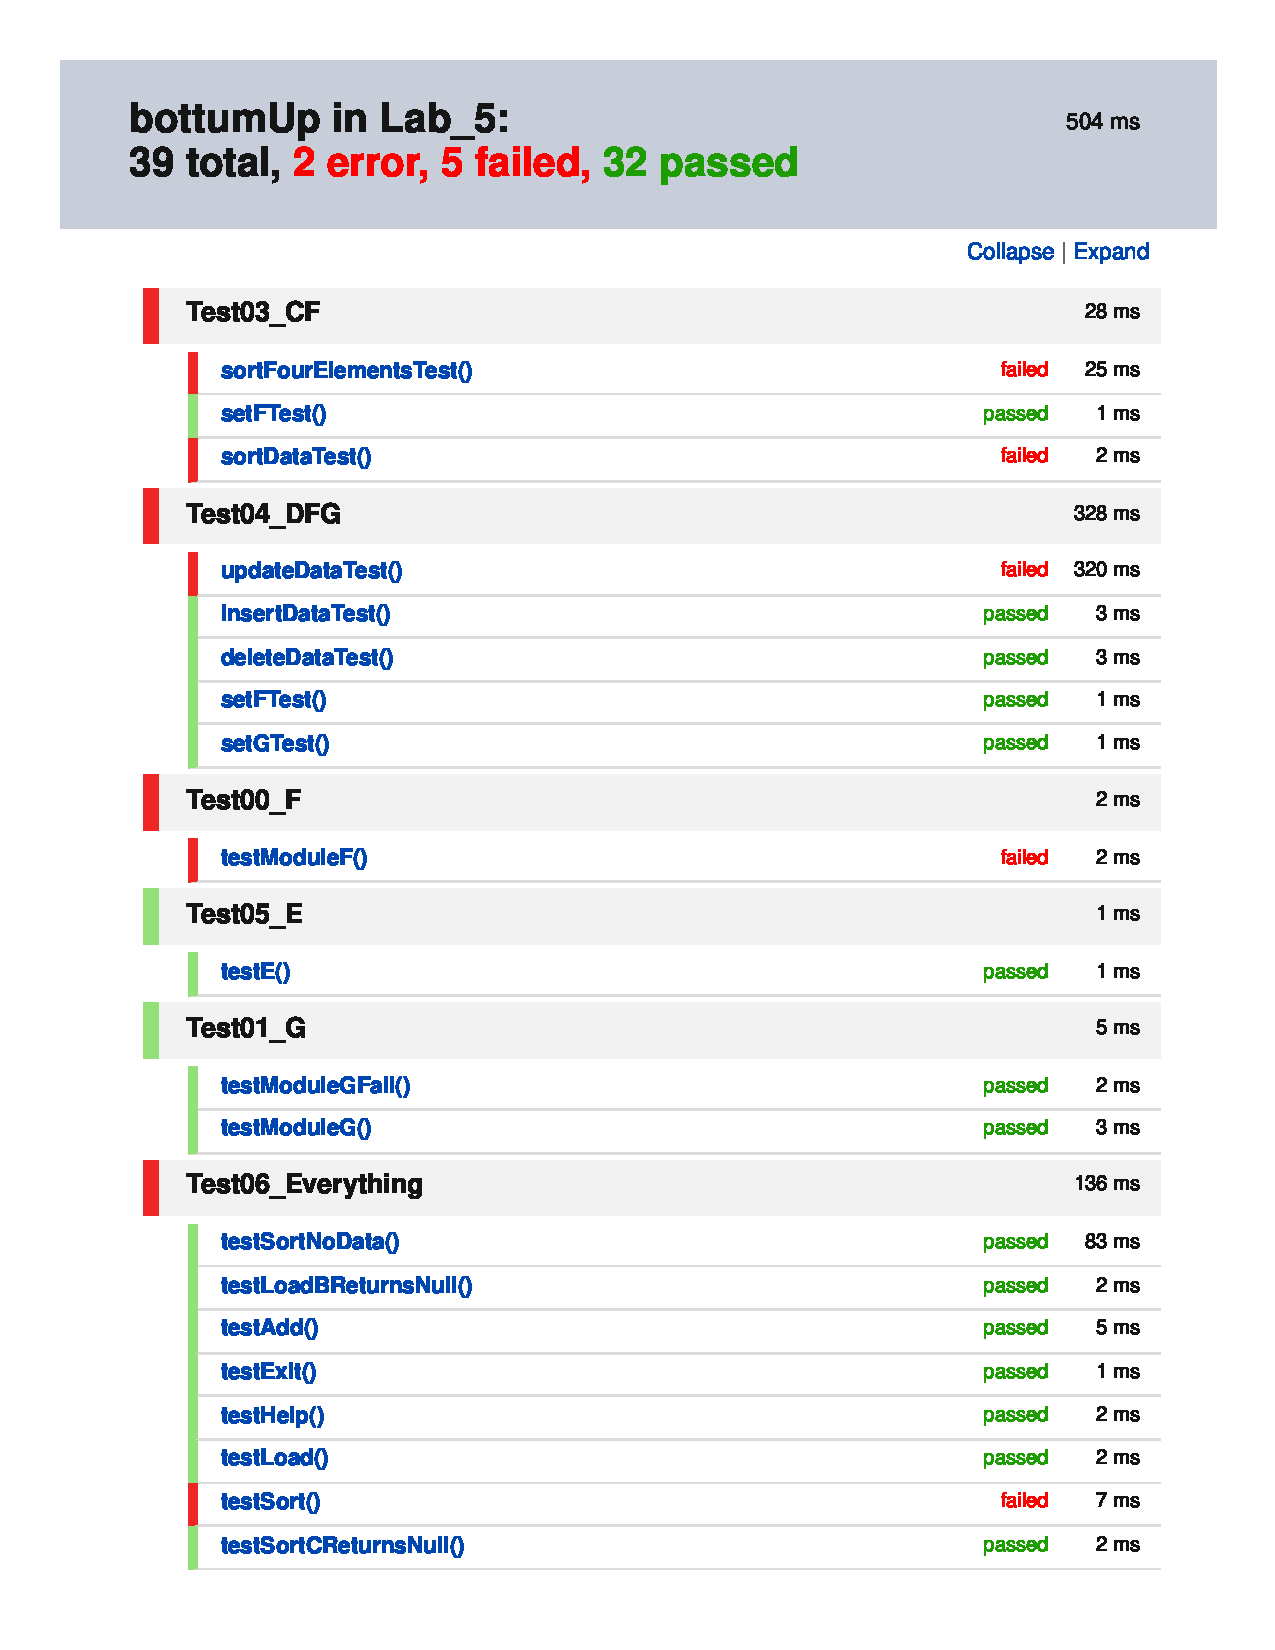
\includepdf[pages=-]{resources/bottomup_results.pdf}

The failing tests are explained as follows:
It should be noted that the tests were run in the order F, G, BF, CF, DFG, E,
Everything.
\subsection{Test CF}
In general, the sorting code appears smelly. It is not using a library function
when one is available for ArrayLists, and the increment variable may not be an
integer number, even though it is being used to help calculate indicies to
manipulate the data. Both of the errors below can be fixed by using the
\textbf{Collections.sort()} method available in java, since \textbf{compareTo()}
for the Entry class is already overridden.
\subsubsection{sortFourElementsTest()}
The application treats the sorting differently for some reason when there are
four elements to sort, because it does a check for when the size of the
collection divided by 2 is equal to 2. In this case, it looks like with four
elements, the application returns an unsorted ArrayList

\begin{verbatim}
Input:
[(ccc, ccc), (aaa, aaa), (bbb, ddd), (bbb, aaa)]
Expected :
[(aaa, aaa), (bbb, aaa), (bbb, ddd), (ccc, ccc)]
Actual :
[(ccc, ccc), (aaa, aaa), (bbb, ddd), (bbb, aaa)]
\end{verbatim}

\subsubsection{sortDataTest()}
The application seems to mostly sort the data ok, but it forgets about sorting
the first element in the data, and leaves it untouched.

\begin{verbatim}
Input    :[(ddd, aaa), (bbb, bbb), (ccc, ccc), (aaa, aaa), (ccc, aaa), (bbb, aaa)]   
Expected :[(aaa, aaa), (bbb, aaa), (bbb, bbb), (ccc, aaa), (ccc, ccc), (ddd, aaa)]
Actual   :[(ddd, aaa), (aaa, aaa), (bbb, bbb), (bbb, aaa), (ccc, aaa), (ccc, ccc)]
\end{verbatim}


\subsection{Test DFG}
\subsubsection{updateDataTest()}
The updateData function takes in an index, but then it adds one to the index.
This results in a test failure when the test expects index 5, for example to be
updated, the application actually ends up updating the entry at index 6.
It is interesting how this unit test fails yet when testing everything at once,
the update command in module A works as expected. Curiously, in module A,
the index is subtracted by 2, so this is probably how the functionality
ends up still working in the end.

\begin{verbatim}
Expected :
[(testName0, testNumber0),
 (testName1, testNumber1),
 (testName2, testNumber2),
 (testName3, testNumber3),
 (testName4, testNumber4),
 (testName, testNumber),
 (testName6, testNumber6),
 (testName7, testNumber7),
 (testName8, testNumber8),
 (testName9, testNumber9)]
Actual :
[(testName0,
 testNumber0),
 (testName1, testNumber1),
 (testName2, testNumber2),
 (testName3, testNumber3),
 (testName4, testNumber4),
 (testName5, testNumber5),
 (testName, testNumber),
 (testName7, testNumber7),
 (testName8, testNumber8),
 (testName9, testNumber9)]
\end{verbatim}

\subsection{Test F}
\subsubsection{testModuleF()}
When Module F displays data, it skips the first line, or the first entry. This
is because the for loop on line 15 in Module F starts from $i=1$, instead of
$i=0$, which means it starts from indexing the second element in the ArrayList,
instead of the first element.

\begin{verbatim}
Expected:
Current Data:
1 name1, number1
2 name2, number2
3 name3, number3
4 name4, number4
5 name5, number5

Actual:
Current Data:
2 (name2, number2)
3 (name3, number3)
4 (name4, number4)
5 (name5, number5)
\end{verbatim}

\subsection{Test Everything}
\subsubsection{testSort()}
This test fails because the file itself is not sorted. Instead, we have a case
where Module A is calling Module C to sort the data, but Module A never tells
another module to update the file with the sorted data, so the database file is
left unmodified and therefore unsorted.

\begin{verbatim}
Input:
ddd,aaa
bbb,bbb
ccc,ccc
aaa,aaa
ccc,aaa
bbb,aaa
Expected :
aaa,aaa
bbb,aaa
bbb,bbb
ccc,aaa,
ccc,ccc
ddd,aaa
Actual :
ddd,aaa
bbb,bbb
ccc,ccc
aaa,aaa
ccc,aaa
bbb,aaa
\end{verbatim}

\subsubsection{testDeleteInvalidArguments()}
The application is not equipped to handle arguments after the delete command
which are non numeric. In such a case where a letter or word is inputted after
the word `delete', the program will ungracefully panic, instead of handling the
error.

\subsubsection{testUpdateInvalidArguments()}
This test fails for the exact same reason for which
testDeleteInvalidArguments() fails.


%general thoughts
